\chapter{Experimenten}

\section{Voorgestelde architectuur}
In deze thesis onderzoeken we of de combinatie van tekstuele data aan de hand van transformermodellen kan omgezet worden in features, die het voorspellingsvermogen van een neuraal netwerk positief beïnvloeden. Ons basisidee ziet er uit zoals beschreven in \autoref{fig:chapt4_architectuur_begin}: eerst worden de geschreven reviews door een transformermodel omgezet naar numerieke features. Deze worden dan toegevoegd aan de input van een neuraal netwerk. We maken dus gebruik van een 'feature augmentation'  hybride model (\ref{sec:chapt2_hybride_modellen}) met machine learning-technieken (\ref{sec:chapt2_machine_learning_modellen}). De overige features voor het neuraal netwerk komen uit de dataset, eventueel verwerkt met feature engineering. Dit betreft dan features die de restaurants beschrijven, zoals het type restaurant (vb.: "fastfood").

\mijnfiguur[H]{width=10.5cm}{fig/chapt4/predictor/architectuur_begin.png}{Schets van de initiële architectuur}{fig:chapt4_architectuur_begin}

Eerst bespreken we hoe we de data gebruiken. In \autoref{sec:chapt4_tekst_naar_features} beschrijven we het onderzoek naar de combinatie van technieken die het best werkt om de geschreven reviews om te zetten naar features voor het neuraal netwerk. In \autoref{sec:chapt4_neuraal_netwerk} leggen we het onderzoek uit naar de optimale vorm van het neuraal netwerk om de verwachte scores zo precies mogelijk te kunnen voorspellen.

\section{Dataflow}
\label{sec:chapt4_data_flow}
Zoals aangeduid in \autoref{fig:chapt4_architectuur_begin}, verwacht het neuraal netwerk vier vectoren als inputdata:
\begin{itemize}
    \item Gebruikersprofiel gecreëerd door NLP (geschreven reviews)
    \item Restaurantprofiel gecreëerd door NLP (geschreven reviews)
    \item Gebruikersprofiel gebaseerd op labels (Yelp dataset labels)
    \item Restaurantprofiel gebaseerd op labels (Yelp dataset labels)
\end{itemize}

Het neuraal netwerk gebruikt deze data om een voorspelling te genereren voor de score die de gespecificeerde gebruiker aan het gespecificeerde restaurant geeft.

\autoref{fig:chapt4_data_flow} toont welke data verwerkt wordt tot profielen, gebruikt wordt voor trainen en welke data gebruikt wordt voor testen. Bij machine learning-technieken is het afgetekend en correct opsplitsen van data in train- en testset uitermate belangrijk. Dit is nodig om de generaliteit van het model te garanderen en overfitting te voorkomen. Door de complexe architectuur van het voorgesteld netwerk is de dataflow niet evident:

\begin{enumerate}
    \item Eerst splitsen we de gebruikers uit de dataset op in twee groepen, steeds met bijhorende reviews voor die gebruikers. De eerste groep stelt de trainset voor, en omvat 80\% van de volledige dataset. De andere groep is de testset, met de overige 20\% van de data.
    \item We gaan eerst verder met de trainset. Het neuraal netwerk verwacht vier vectoren, die steeds een gebruikersprofiel of restaurantprofiel voorstellen. Echter kunnen we niet gewoon alle reviews van een gebruiker verwerken om deze profielen op te stellen! 
    
    Indien we dat wel zouden doen, zouden de gegevens van de te voorspellen review verwerkt worden in het profiel. Als we later het model trainen op deze review, bevat de profielvector gegevens over de gebruiker die we op dat punt nog niet zouden mogen weten. We zouden dus trainen op data die in een echte gebruikersomgeving nog niet beschikbaar is.

    We splitsen daarom de trainset nogmaals op in twee delen door willekeurig de reviews te samplen. De eerste set stelt dan de geschiedenis voor van een gebruiker of restaurant, en wordt strikt gebruikt om gebruikers- en restaurantprofielen op te stellen. Dit omvat 70\% van de reviews uit de trainset.\newline
    De overige 30\% van de reviews wordt gebruikt om het neuraal netwerk te trainen: we linken de gebruiker en het restaurant van die reviews met de bijhorende profielen gemaakt in het eerste deel. Dit stelt de input van het neuraal netwerk voor. De score van die reviews uit het tweede deel stelt de output voor. Hiermee hebben we dus alle informatie om het neuraal netwerk te trainen. 

    \item Na het trainen van het neuraal netwerk, wordt analoog aan stap 2 ook de testset verwerkt tot profielen en ongeziene reviews. Deze worden dan gebruikt om te meten hoe goed het model in staat is om aan de hand van de profielen een score te voorspellen.

    \item Er wordt enkele keren met dezelfde profielen en dezelfde ongeziene reviews getraind. Doordat de profielen niet steeds opnieuw moeten uitgerekend worden, gaat het verwerken van deze epochs sneller.

    \item Na iedere $k$ epochs worden dezelfde train- en testset opnieuw opgedeeld tot data voor profielen en ongeziene reviews. Hierdoor kunnen we de volledige dataset efficiënter benuttigen.
\end{enumerate}


\mijnfiguur[H]{width=17cm}{fig/chapt4/predictor/data_flow.png}{Schets van dataflow doorheen het model}{fig:chapt4_data_flow}

\section{Tekst naar features}
\label{sec:chapt4_tekst_naar_features}
In deze sectie zullen we beschrijven hoe we uit de tekstuele reviews features (profielen) zullen verkrijgen die we gebruiken als input voor het neuraal netwerk. Ook beschrijven we de redeneringen achter de algoritmen, met andere woorden wat deze features moeten voorstellen. We zullen deze algoritmen hoofdzakelijk baseren op BERTopic. We onderzoeken de capaciteiten van verschillende modellen, en trachten deze zo objectief mogelijk te evalueren. BERTopic zal de reviews opsplitsen in clusters. Voordat we de reviews kunnen gebruiken als inputvector voor het neuraal netwerk, moeten we deze clustering eerst nog omzetten tot gebruikers- en restaurantprofielen. Dit proces is ook gevisualiseerd in \autoref{fig:chapt4_structuur_evaluatie_bertopic}.

\mijnfiguur[H]{width=16cm}{fig/chapt4/NLP/structuur_evaluatie_bertopic.jpg}{Tekstuele reviews omzetten naar gebruikers- en restaurantprofielen}{fig:chapt4_structuur_evaluatie_bertopic}

\subsection{Testset-up}
\label{sub:chapt4_testsetup}
We hebben gebruik gemaakt van een bestaande implementatie van BERTopic \cite{bertopic_homepage} waarbij we de verschillende lagen aanpassen. We gebruiken sentence-BERT van sentence-transformers. \cite{sentence_transformers_implementation} Zoals gevisualiseerd in \autoref{fig:chapt4_structuur_evaluatie_bertopic} kunnen we ons algoritme op meerdere plaatsen evalueren. In volgende paragrafen zullen we beide manieren met elkaar vergelijken.

\subsubsection{Evaluatie van profielen}
\label{sub:chapt4_evaluatie_profielen}
Een eerste mogelijkheid is om de uiteindelijk verkregen profielen te evalueren. Aan de ene kant modelleren deze wat een bepaalde gebruiker belangrijk vindt via het gebruikersprofiel. We combineren dit met een restaurantprofiel: dit stelt de specialiteiten en andere eigenschappen van een bepaald restaurant voor. Om deze profielen te evalueren, zullen we gebruik maken van de architectuur afgebeeld in \autoref{fig:chapt4_architectuur_begin}. Hierbij zullen we het volledige neuraal netwerk constant houden met uitzondering van deze NLP-profielen. We gebruiken een beperkt aantal epochs om sneller resultaten te verkrijgen. De precieze implementatie staat uitgeschreven in \autoref{sec:chapt4_basisimplementatie}. We kiezen dan de beste combinatie van profielen op basis van minimale loss door een grid search uit te voeren over alle mogelijke combinaties. We letten ook op de trend van de loss, om zeker te zijn dat er geen significante verschillen meer zullen optreden als we het model trainen met meer epochs. Op deze manier kunnen we de performantie van de profielen objectief beoordelen.

\subsubsection{Evaluatie van de clustering}

De tweede evaluatietechniek werkt aan de hand de verkregen clusters zoals beschreven in \autoref{sub:chapt2_bertopic_clustering}. Bij de keuze van een evaluatiemetriek voor deze clusters moeten we rekening houden met enkele aspecten. Het eerste is dat we geen gelabelde data hebben. In theorie kunnen we de zinnen handmatig labelen aan de hand van een lijst van topics. Dit introduceert een eerste vorm van subjectiviteit in de evaluatie, daar de zinnen anders geïnterpreteerd kunnen worden dan oorspronkelijk bedoeld, of het toekennen van een topic ambigu kan zijn. Hierbij stelt zich een bijkomend probleem dat elk BERTopic-model verschillende topics zal maken, met als gevolg dat iedere zin voor ieder model apart zal moeten gelabeld worden. Door deze redenen zullen we metrieken die gebruik maken van de ground truth-labels uitsluiten en gebruik maken van de technieken beschreven in \autoref{sec:chapt2_clustering_evaluation}.

Met de overige technieken kunnen we de verschillende modellen vergelijken. Het doel van deze evaluatiemethode is om een idee te krijgen hoe goed de clustering werkt, onafhankelijk van een neuraal netwerk. Een bijkomend voordeel is dat deze metrieken dus minder computationeel intensief zijn dan het trainen van een neuraal netwerk.

\subsection{Clustering via BERTopic}
In deze sectie bespreken we hoe we BERTopic gebruiken om een clustering te genereren. Deze modellen gebruiken we dan bij het creëren van gebruikers- en restaurantprofielen in \autoref{sec:chapt4_nlp_profielen}. Merk op dat het gebruikte embeddingmodel bij BERTopic getraind is op algemene data. Idealiter beschikken we over een gelabelde dataset die specifiek in context van de culinaire wereld kan aangeven hoe gelijkaardig twee zinnen zijn. Helaas is dit niet het geval, waardoor finetunen van het sentence-BERT model niet mogelijk is. Hierdoor verwachten we dat de interclusterafstand relatief laag zal zijn, daar een algemeen model alle topics rond \q{eten} moeilijker zal kunnen onderscheiden.

\subsubsection{Aanpassingen BERTopic}
Het initiële model zal gebruik maken van de standaardimplementatie, zoals beschreven in \autoref{sub:chapt2_bertopic}, in combinatie met sentence-BERT. Deze implementatie is voor de volledigheid gevisualiseerd in \autoref{fig:basismodel_bertopic}. Bovenop dit model zullen we ook nog een extra finetuning-laag toevoegen, namelijk KeyBERTInsipired beschreven in \autoref{sub:topic_representatie}

\mijnfiguur[H]{width=5cm}{fig/chapt4/NLP/basismodel_bertopic.jpg}{Visualisatie van de standaardimplementatie van BERTopic \cite{bertopic_algo}.}{fig:basismodel_bertopic}

De eerste stap is het bepalen wat de documenten zullen voorstellen. Hiervoor hebben we meerdere mogelijkheden: de meest voor de hand liggende mogelijkheid is dat we iedere review als een afzonderlijk document beschouwen. Dit zal betekenen dat we ongeveer 4,7 miljoen documenten hebben. Deze aanpak heeft enkele complicaties:

Door het gebruik van BERTopic zoals beschreven in \autoref{sub:chapt2_bertopic} kunnen we een document maar aan één cluster toevoegen. Dit is tegenstrijdig met de realiteit, waar reviews meerdere onderwerpen aankaarten zoals \q{lekker eten} maar \q{slechte service}. Aangezien een cluster overeenkomt met precies één onderwerp, is dit geen ideale match. We kunnen deze complicatie deels vermijden door de reviews op te splitsen in zinnen. Dit zal gebeuren via een sentence tokenizer zoals beschreven in \autoref{sub:chapt2_tokenization}. Hierbij veronderstellen we wel nog steeds dat één zin overeenkomt met één onderwerp. Gebaseerd op een steekproef lijkt dit voor de meeste zinnen uit de reviews wel een correct besluit. Onze implementatie gebruikt de sentence tokenizer van SpaCy. \cite{spacy_main}

Hieruit volgt een nieuwe uitdaging: schaalbaarheid. Het clusteren van 36 miljoen in-memory documenten is niet triviaal. De vereiste hoeveelheid werkgeheugen zal nog toenemen eens we een clustering creëren. Voor ongeveer 2\% van de data (100 000 reviews $\approx$ 700 000 documenten) is dit nog net mogelijk met 64GB werkgeheugen. We kunnen het BERTopic-model opstellen met deze subset en vervolgens de overige 98\% bevragen aan de hand van dit getrainde model.\newline
De volledige dataset zou geschat 3TB werkgeheugen nodig hebben om alle reviews te clusteren volgens het standaard BERTopic-algoritme.

We groeperen dus elke van de 36 miljoen zinnen in een cluster op basis het BERTopic-model getraind op slechts 2\% van de data. Hierdoor zijn we in staat om meerdere onderwerpen aan één review toe te kennen. Voor de rest van deze masterthesis zullen we één document gelijkstellen aan één zin uit een review.

Een bijkomend nadeel van deze methode is dat sommige zinnen uit geen enkel relevant onderwerp bestaan. Dit zijn zinnen die, ongerelateerd aan het restaurant, een verhaal vertellen of bepaalde omstandigheden omschrijven. Het gevolg kan waargenomen worden in de representatie van enkele topics, zoals \q{traffic} of \q{sunny}.



\subsubsection{Online BERTopic}
Een online algoritme, ook wel incrementeel algoritme genoemd, is een algoritme dat gebruik kan maken van een datastroom zonder de volledige input te weten. Hierdoor kan het algoritme de data in kleinere delen verwerken. Deze techniek is toepasbaar op BERTopic, wat in ons geval interessant is. Een bijkomend voordeel hiervan is de mogelijkheid om toekomstige data efficiënt te verwerken. In een productieomgeving worden steeds nieuwe reviews gemaakt. Omdat we het model incrementeel kunnen updaten met nieuwe data, hoeven we niet een volledig nieuw BERTopic model te maken om deze data te verwerken.\newline
In ons onderzoek met een statische dataset is dit niet relevant, maar dit is zeker een nuttige eigenschap voor een productieomgeving.

Om BERTopic om te zetten naar een online algoritme, zullen we alle stappen moeten omzetten naar een online variant, indien dit nog niet het geval is. Hoe deze stappen omgezet worden, staat hieronder beschreven. Deze transformatie wordt ook gevisualiseerd in \autoref{fig:chapt4_bertopic_online_transformation}

\begin{itemize}
    \item \textbf{De embedding} komt uit een LLM. Dit LLM hoeft niet continu getraind te worden en kan al bevraagd worden voor ongeziene data. Door de generaliteit van het LLM is er dus geen aanpassing nodig.
    \item Voor \textbf{dimensionaliteitsreductie} gebruiken we een online variant, namelijk Incremental PCA (IPCA).
    \item Bij het \textbf{clusteringsalgoritme} schakelen we over naar een online K-Means algoritme: MiniBatch K-Means.
    \item \textbf{De BOW representatie} wordt ook aangepast naar zijn online variant.
    \item Aangezien \textbf{c-TF-IDF} en verdere aanpassingen gebaseerd zijn op de data van de BOW representatie zal hier geen verdere aanpassing nodig zijn.
\end{itemize}

\mijnfiguur[H]{width=12cm}{fig/chapt4/NLP/bertopic_to_online.jpg}{Transformatie van de standaard BERTopic-structuur naar een online algoritme.}{fig:chapt4_bertopic_online_transformation}

Door het gebruik van deze structuur kunnen we het model op een grotere hoeveelheid data trainen. We hebben dus een schaalbare implementatie gecreëerd. De trainingstijd van dit model zal lineair stijgen op basis van de grootte van de trainingsdata. Als input kunnen we voor dit model de volledige dataset gebruiken. Dit komt omdat we hier geen rechtstreekse features genereren voor het neuraal netwerk, maar slechts een lijst van \textit{mogelijke} topics opstellen.

\subsubsection{Guided BERTopic}
Een laatste experiment voor clustering maakt gebruik van guided BERTopic \cite{bertopic_guided}, een reeds geïmplementeerde variant op het standaardalgoritme. Hierbij geven we per topic een lijst van woorden mee die dit topic beschrijven. Deze lijst van woorden wordt de seed van de topic genoemd. Het uiteindelijke model houdt hiermee rekening en zal de kans vergroten om deze seeded topics als finale output te genereren. Merk op dat dit volgens de auteur niet altijd het geval is. Vaak zullen deze topics aangepast of opgesplitst worden, tenzij deze extreem accuraat zijn.

We stellen hiervoor manueel een lijst van woorden op, gegroepeerd per topic. De keuze van de woorden is gebaseerd op de categorieën uit de Yelp Dataset. We vermelden dat deze topics zeer subjectief gekozen zijn. De opdeling staat in \verb|src/NLP/guided_topics.txt|.

Via deze methode willen we het probleem van irrelevante topics, als gevolg van het opsplitsen in zinnen, vermijden. We doen dit door naast de vaste lijst van topics, het model ruimte te geven om extra topics te genereren. Het doel is dat deze extra topics gevuld worden met de irrelevante zinnen.

Na enkele pogingen met verschillende parameters zien we steeds hetzelfde probleem opduiken: door de grote hoeveelheid data worden de voorgedefinieerde topics overspoeld met andere data. Hierdoor blijft er weinig over van de originele seeds. Een mogelijke oplossing is om minder data te gebruiken. Hierdoor kunnen we ook gebruik maken van de standaardimplementatie van BERTopic. Door minder data te gebruiken zijn de resultaten echter significant slechter, wat we verder bespreken in \autoref{sub:chapt5_nlp_resultaten}.

\subsubsection{Optimalisaties}
% cache => bijhouden
% append only => dus niet vaak herberekenen (enkel als model veranderd)
% schaalbaar => in praktijk ook nuttig
Aangezien we het model vaak zullen bevragen met dezelfde data tijdens het trainen van het neuraal netwerk, is het mogelijk om voor ieder document op voorhand het topic uit te rekenen. De resultaten kunnen dan opgeslagen worden op de harde schijf. Tijdens het trainen van het neuraal netwerk kunnen de resultaten snel ingelezen worden voor bevraging. Merk op dat reviews in een productieomgeving zelden wijzigen: er worden hoofdzakelijk enkel nieuwe reviews toegevoegd. Dit maakt het precomputen van de topics nog aantrekkelijker, want het inlezen van een bestand duurt minder lang dan het bevragen van het model. Hierdoor is het idee van het omzetten van zinnen naar topics haalbaar om in realtime aanbevelingen te maken.

\subsection{Evaluatie clustering}
\label{sub:chapt4_eval_clustering}
Voordat we verder gaan met deze modellen om gebruikers- en restaurantprofielen te genereren, gaan we voor iedere implementatie een evaluatie op de clustering uitvoeren. We doen dit door de clusteringsmetrieken, beschreven in \autoref{sec:chapt2_clustering_evaluation}, uit te rekenen. Aangezien de meeste metrieken niet schaalbaar zijn, gebruiken we slechts een deel van de data voor de berekeningen. Om te bepalen hoe groot dit deel moet zijn om representatieve scores te behalen, vergelijken we eerst dezelfde metrieken over hetzelfde model, maar met een verschillende hoeveelheid data.

\begin{figure}[H]
    \begin{subfigure}{.5\textwidth}
        \centering
        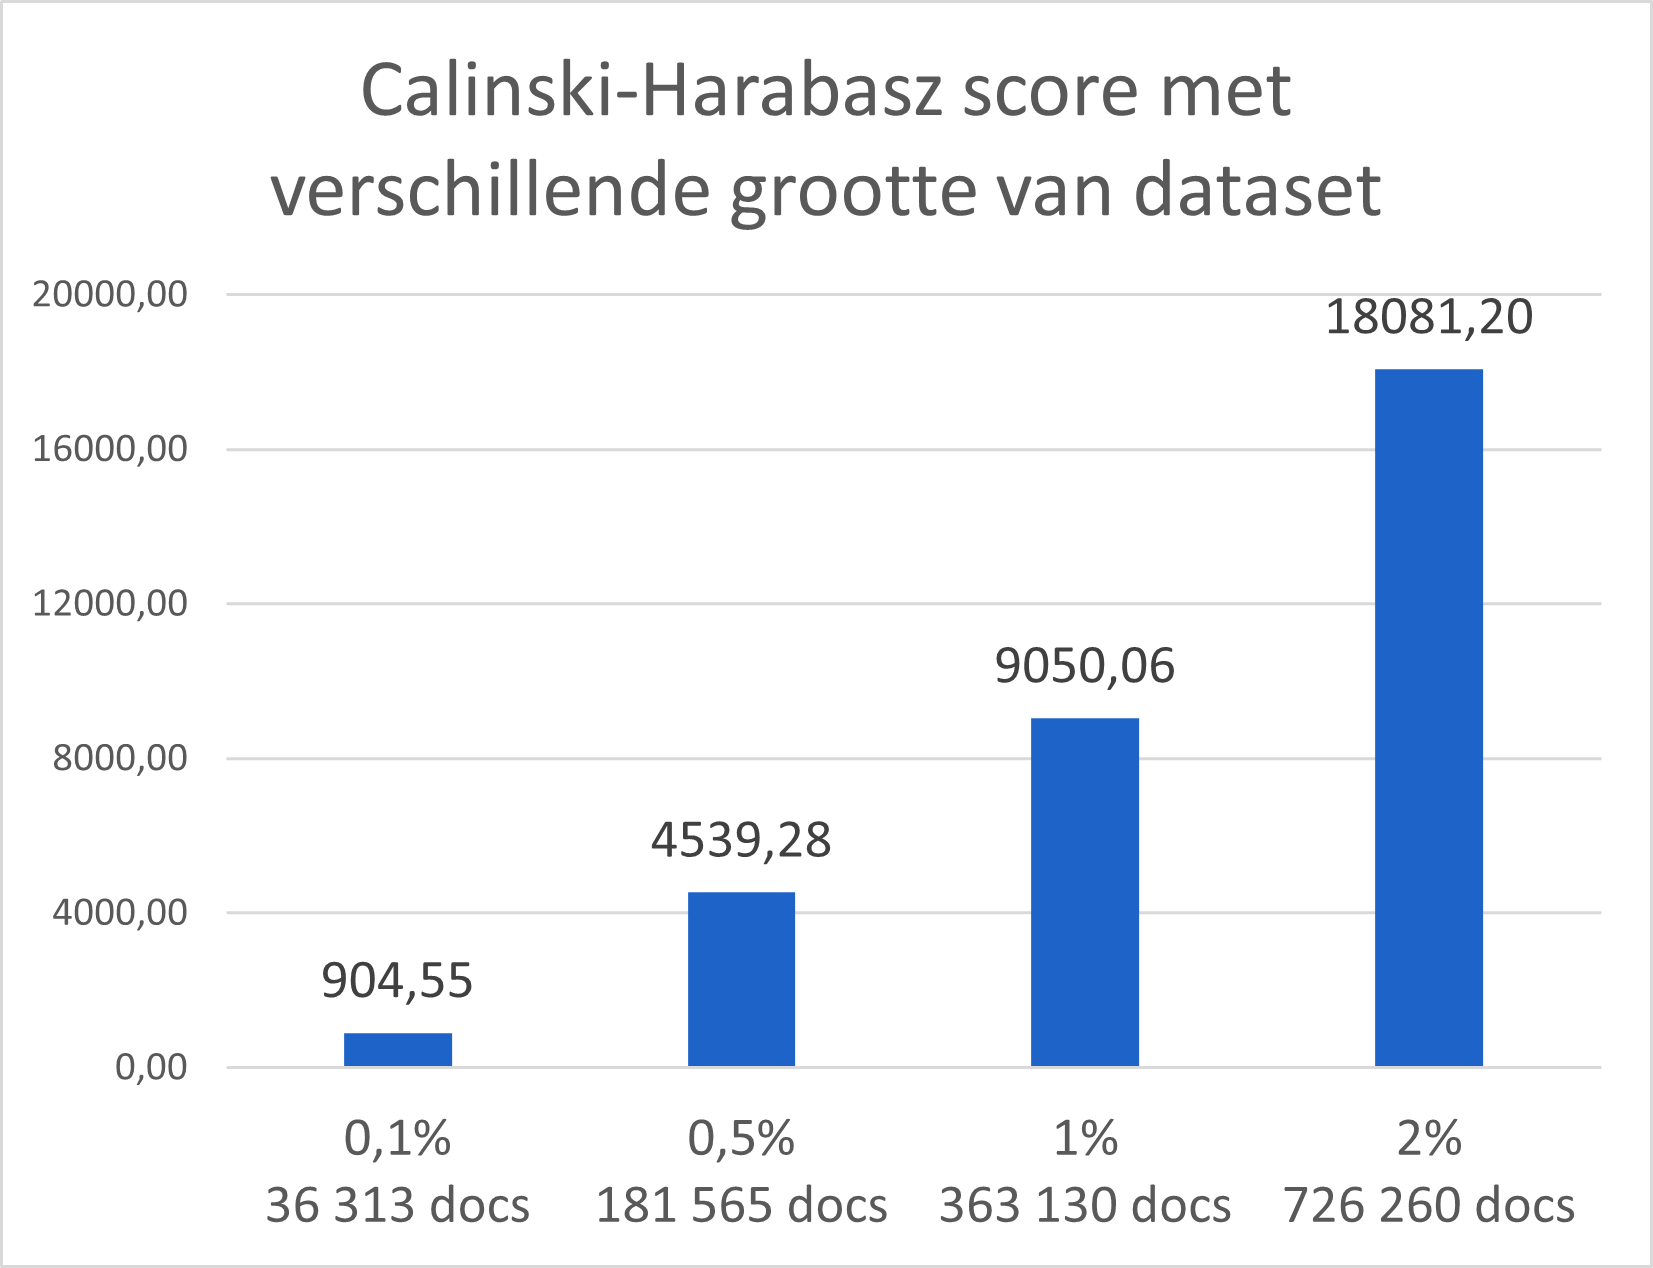
\includegraphics[width=1\linewidth]{fig/chapt4/NLP/cal_data.png}
    \end{subfigure}
    \begin{subfigure}{.5\textwidth}
        \centering
        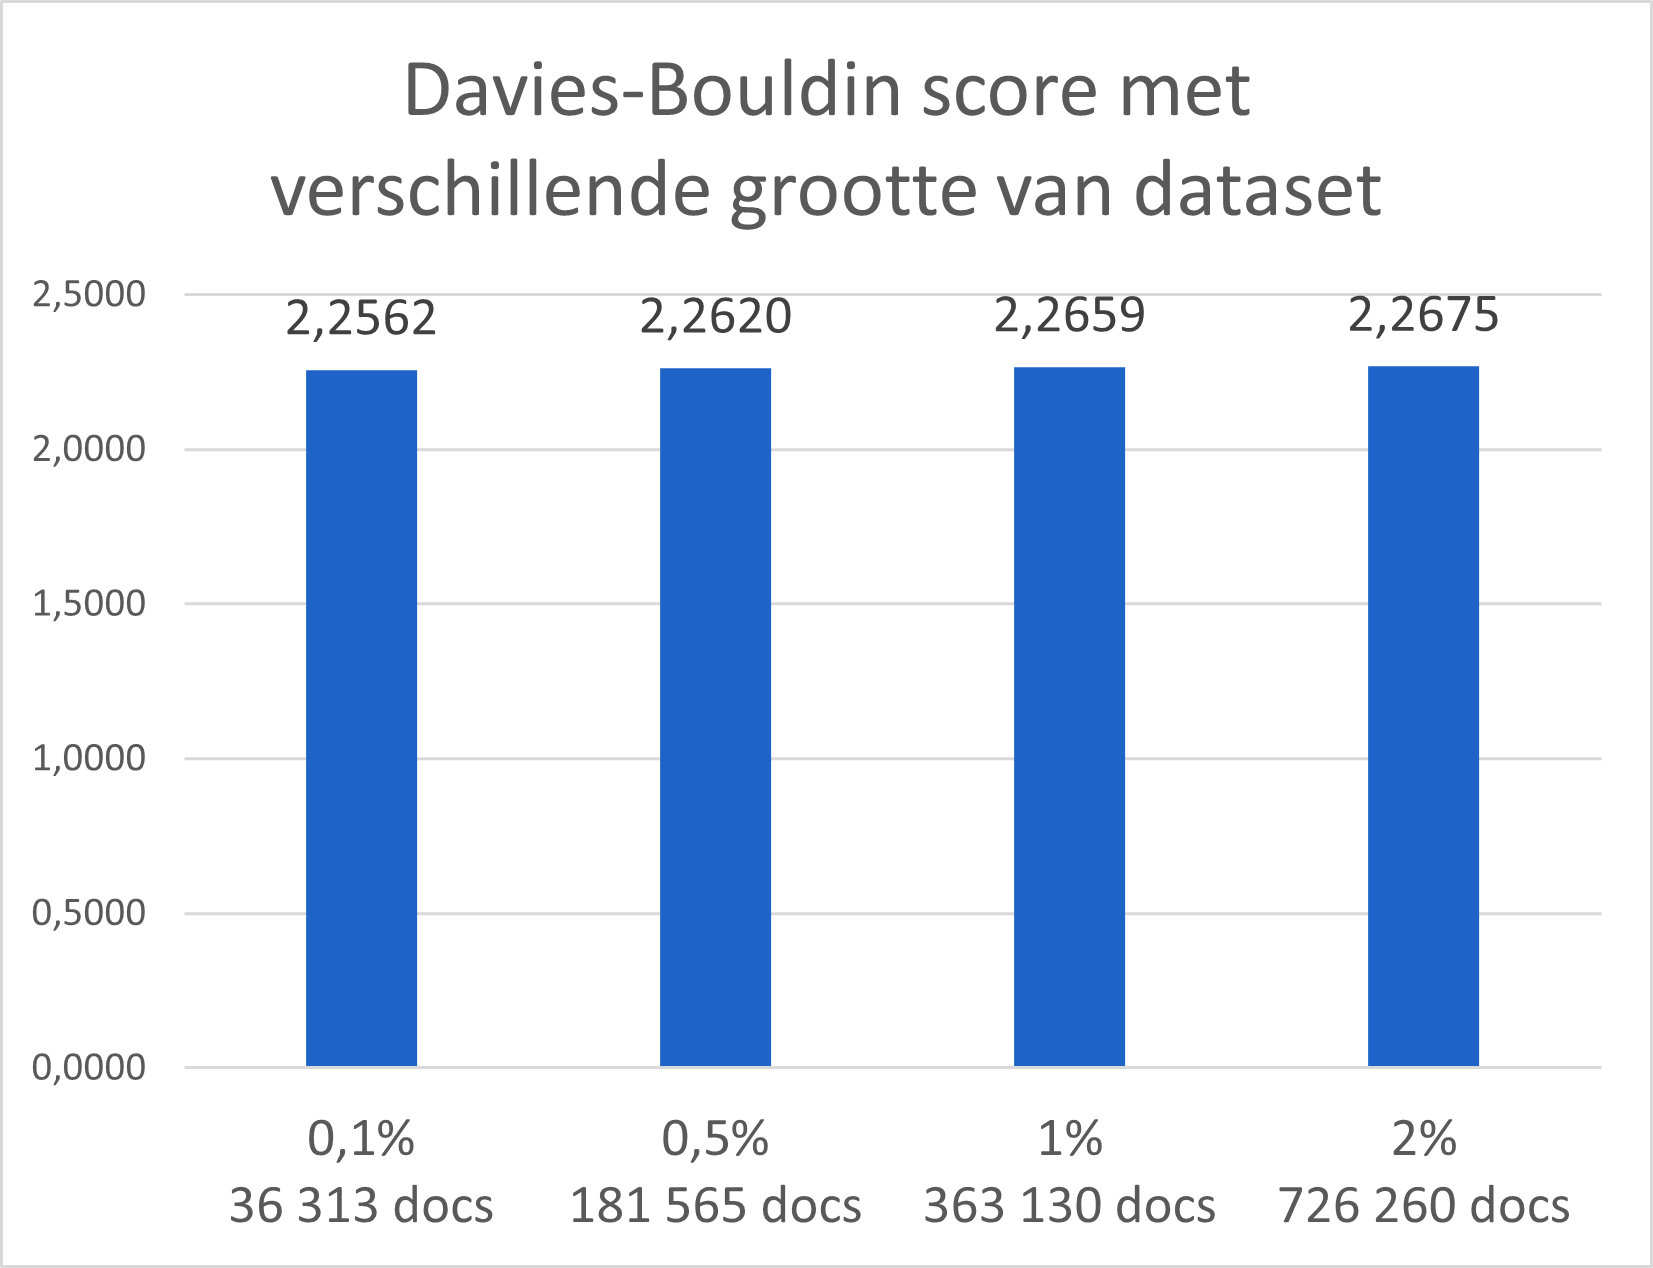
\includegraphics[width=1\linewidth]{fig/chapt4/NLP/davies_data.png}
    \end{subfigure}
    
    \centering
    \begin{subfigure}{.5\textwidth}
        \centering
        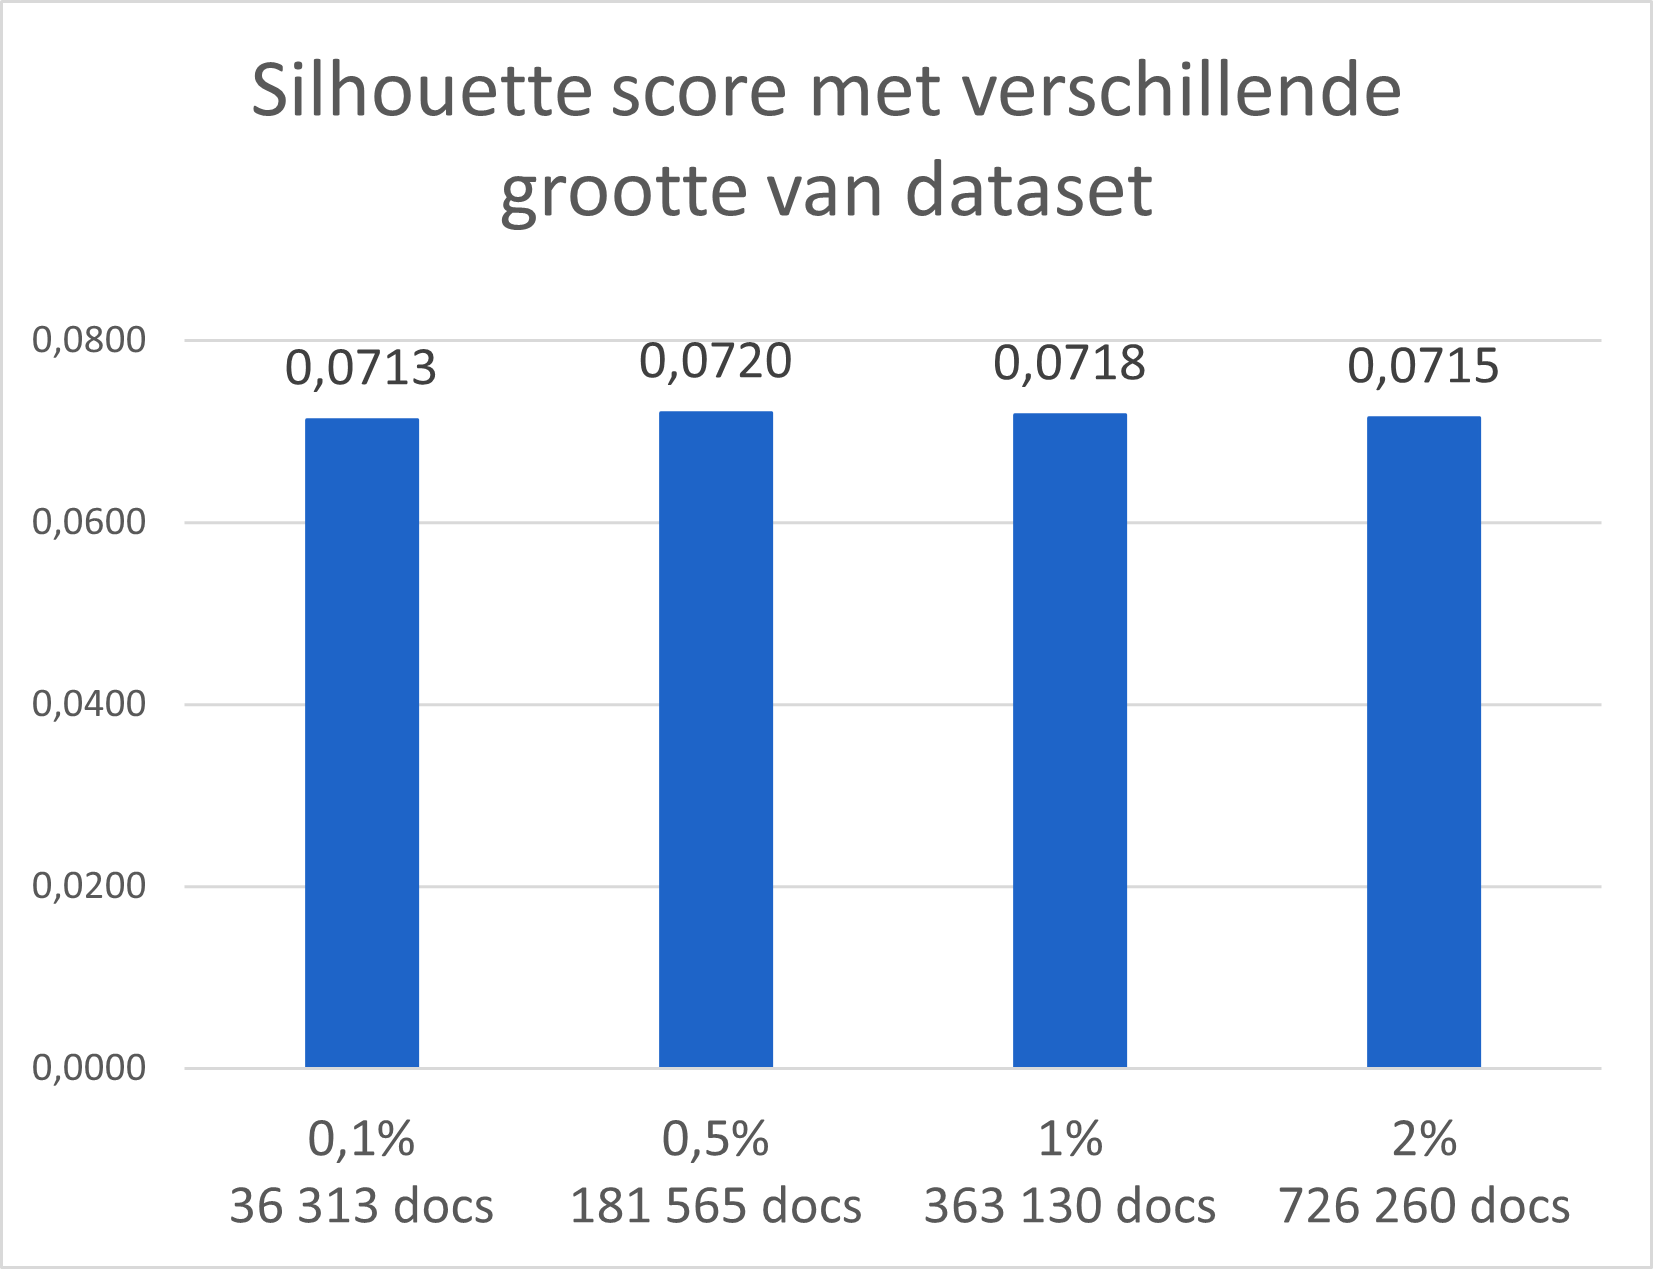
\includegraphics[width=1\linewidth]{fig/chapt4/NLP/silhouette_data.png}
    \end{subfigure}
    \caption{De scores van het model online\_50, voor verschillende groottes van de dataset}
    \label{fig:chapt4_datapercentage_clusteringmetrics}
\end{figure}

In \autoref{fig:chapt4_datapercentage_clusteringmetrics} zijn de scores weergegeven voor $0,1\%$, $0,5\%$, $1\%$ en $2\%$ van de dataset. We kunnen waarnemen dat er geen significante verschillen zijn voor de Davies-Bouldin score en silhouette score. Voor de Calinski-Harabasz score zien we een lineaire stijging die afhangt van de hoeveelheid data. Deze stijging is te verklaren door het gebruik van het aantal datapunten in de formule. Doordat de metrieken de eigenschappen van de clusters modelleren, concluderen we dat er geen significante verschillen tussen de clusterings zijn bij verschillende datagroottes, en dat de metrieken over een subset van de datapunten representatief zijn voor alle datapunten. In de volgende vergelijkingen gebruiken we daarom enkel de scores van $1\%$ van de data. 

\begin{figure}[H]
    \begin{subfigure}{.5\textwidth}
        \centering
        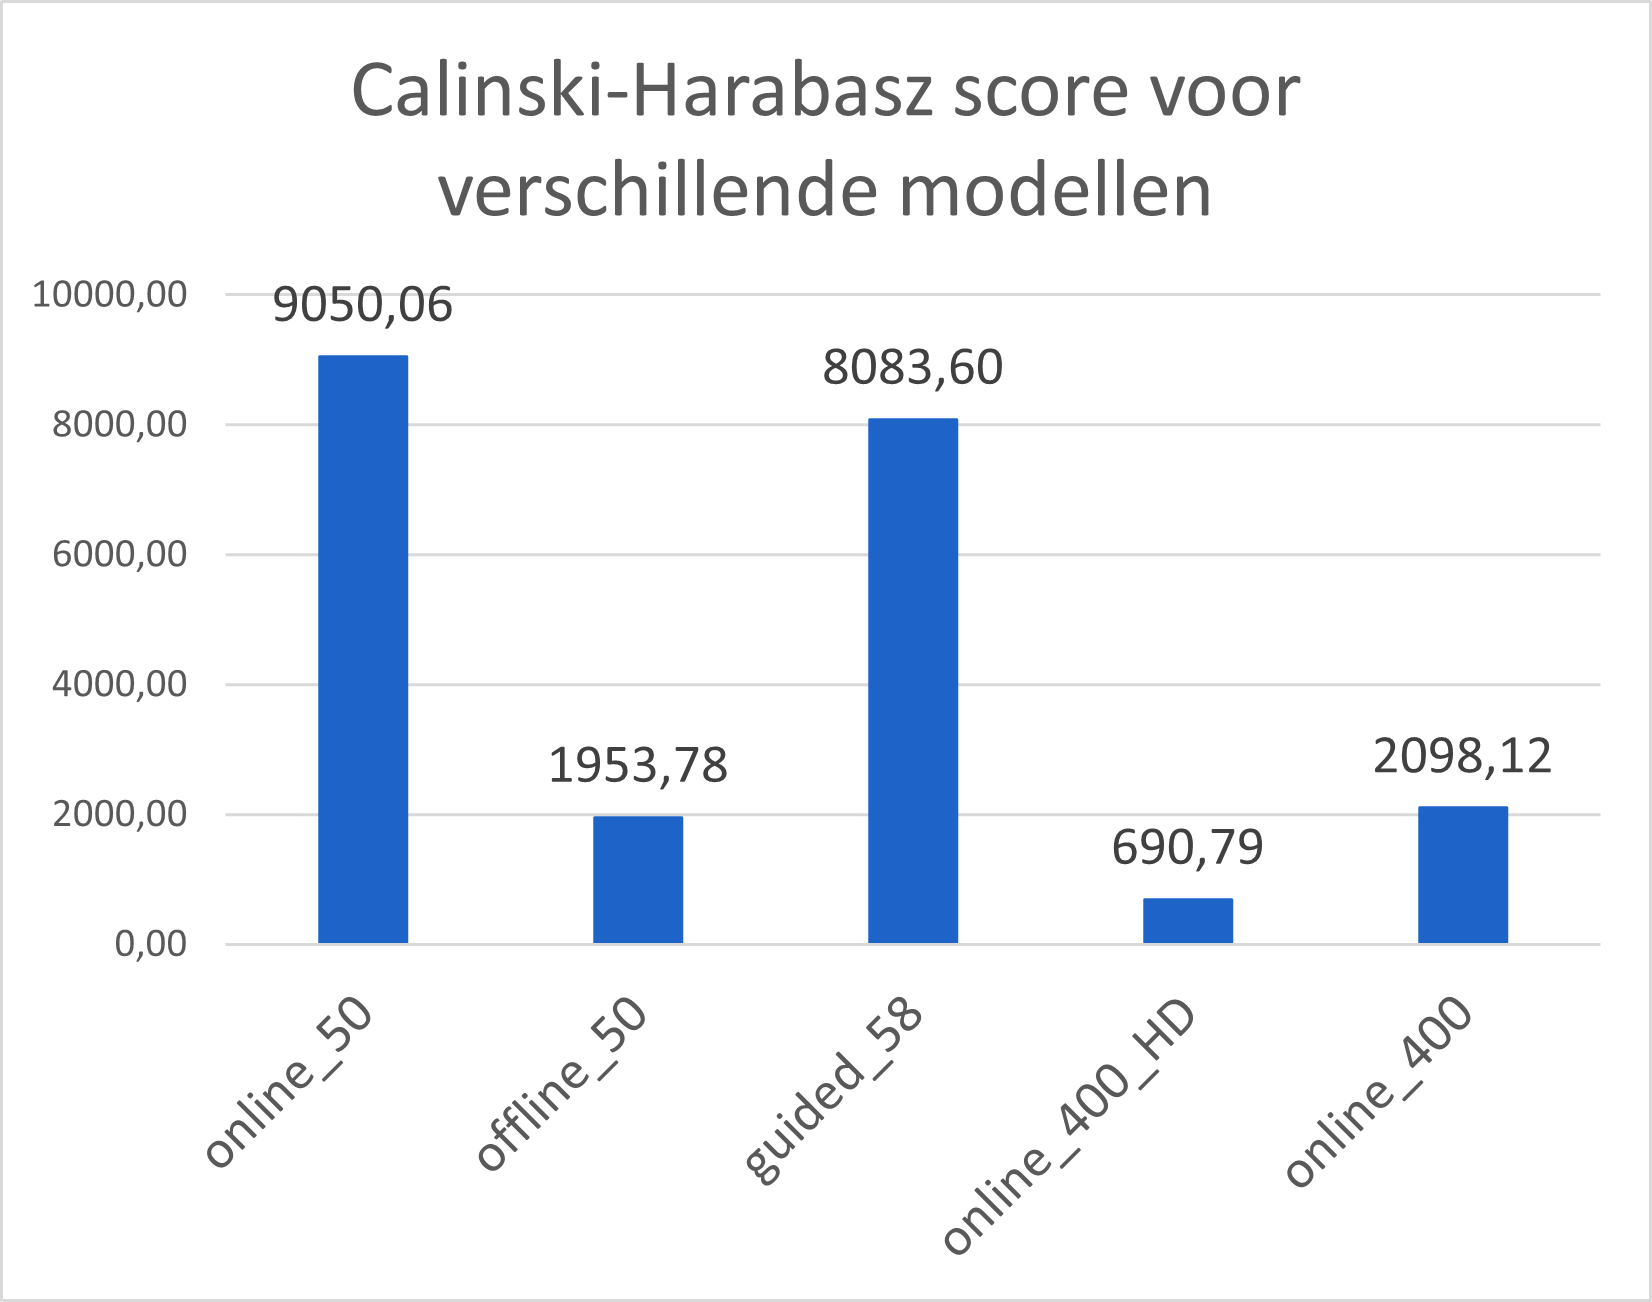
\includegraphics[width=1\linewidth]{fig/chapt4/NLP/cal_model.png}
    \end{subfigure}
    \begin{subfigure}{.5\textwidth}
        \centering
        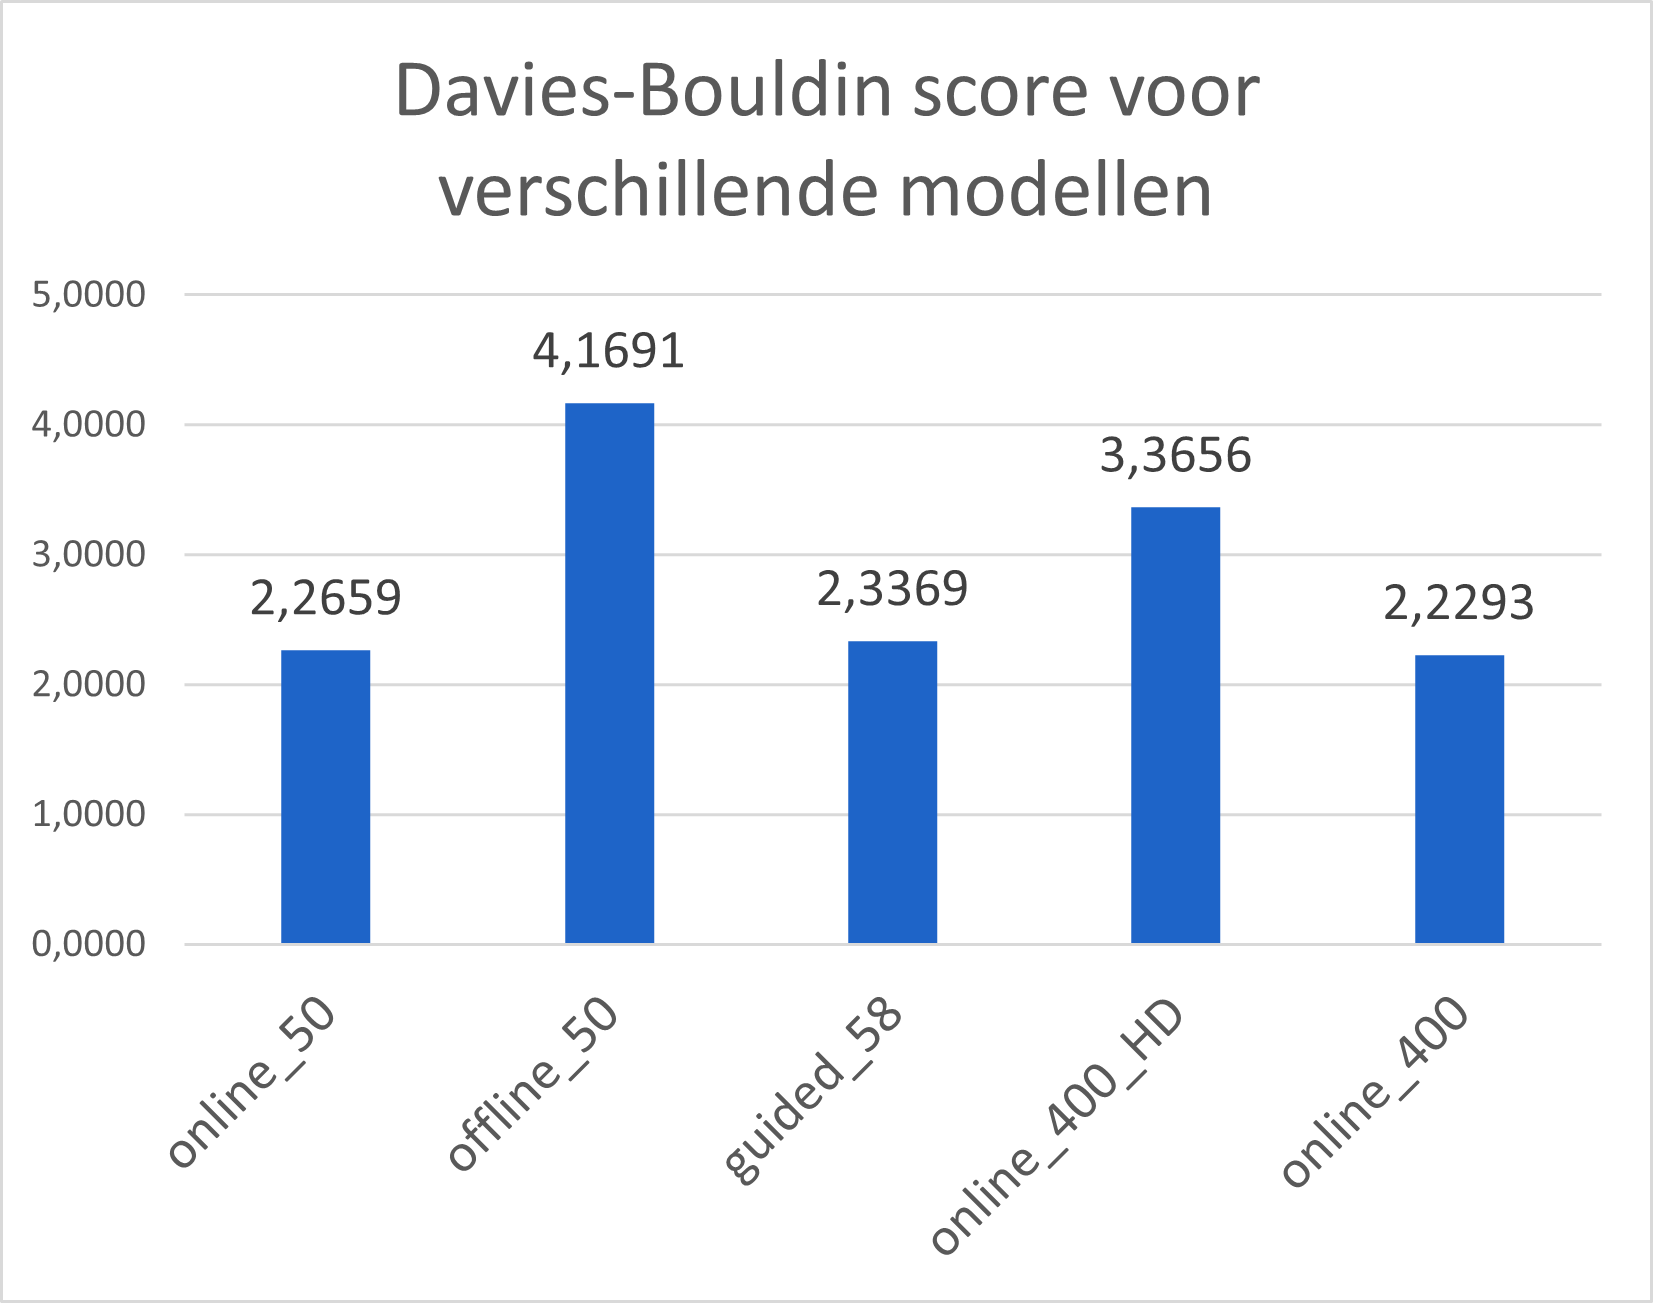
\includegraphics[width=1\linewidth]{fig/chapt4/NLP/davies_model.png}
    \end{subfigure}
    
    \centering
    \begin{subfigure}{.5\textwidth}
        \centering
        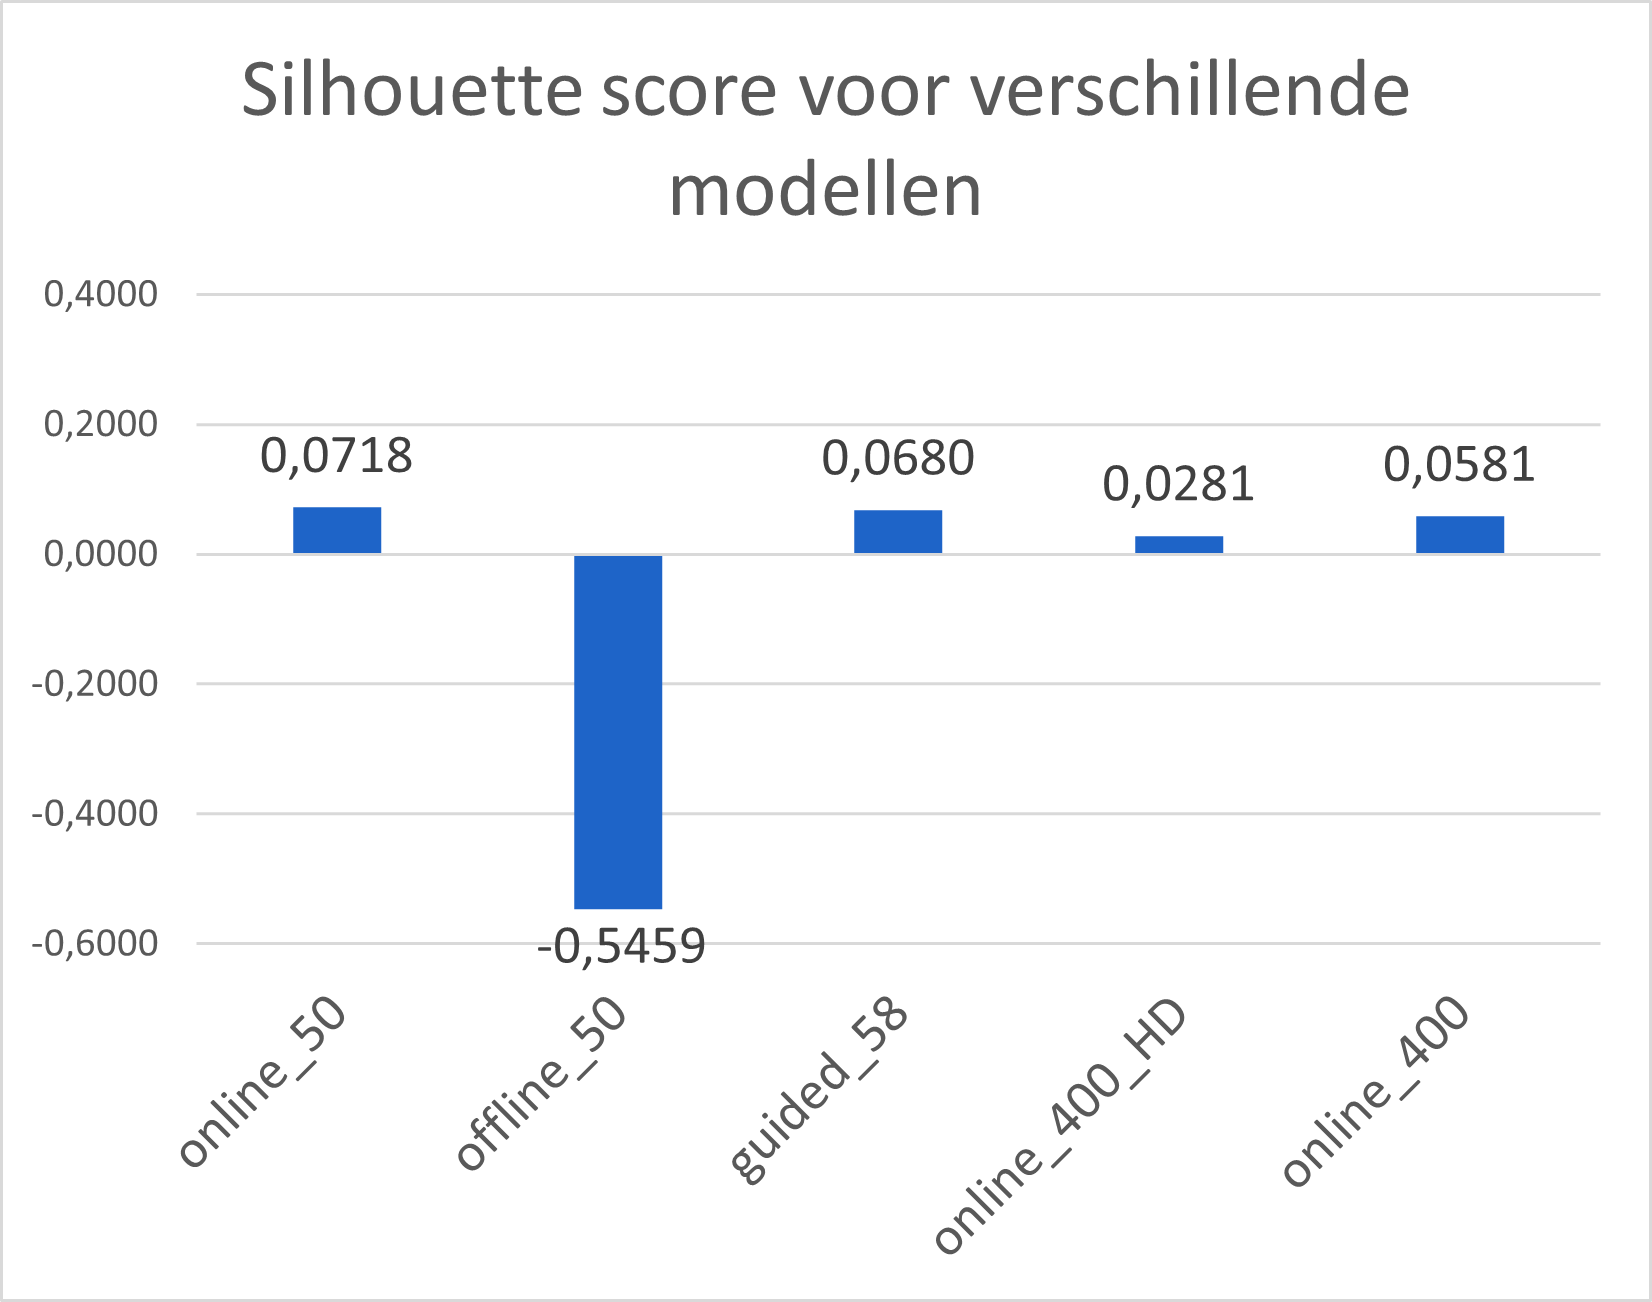
\includegraphics[width=1\linewidth]{fig/chapt4/NLP/silhouette_model.png}
    \end{subfigure}
    \caption{Scores voor de verschillende modellen (1\% van dataset)}
    \label{fig:chapt4_clusteringmetrics_vergelijking}
\end{figure}

Uit \autoref{fig:chapt4_clusteringmetrics_vergelijking} kunnen we het volgende concluderen: de volgende modellen hebben algemeen de beste scores: online\_50, online\_400 en guided\_58\footnote{\q{online\_50} wil zeggen \q{Online BERTopic, 50 topics}, etc}. Voor deze modellen liggen de Davies-Bouldin score en silhouette score dicht bij elkaar. De exacte volgorde verschilt afhankelijk van de gekozen metriek. In het geval van Calinski-Harabasz score zijn er verschillen, maar deze linken we aan het verschillend aantal topics per model.\newline
Het vierde beste model is online\_400\_HD waarbij de dimensionaliteitsreductie meer dimensies behoudt. Hierbij zien we dat de silhouette score iets slechter is, maar de Davies-Bouldin score significant hoger en dus slechter is. Voor de Calinski-Harabasz score kunnen we het enkel vergelijken met een ander model van 400 topics, namelijk online\_400. Hierbij nemen we waar dat de score significant lager en dus slechter is. Het laatste model is offline\_50, hierbij zien we dat alle scores significant slechter zijn. Merk op dat de silhouette score zelfs sterk negatief is wat wijst op een slechte clustering.

Voor de drie beste modellen geven de scores aan dat de clustering niet optimaal is, maar dit betekent niet dat er een betere clustering is. Deze metrieken moeten we vooral gebruiken om verschillende clusteringsalgoritmen te vergelijken. Een potentiële verklaring kan zijn dat sentence-BERT, het model gebruikt voor de embeddings te generen, getraind is op algemene data en dus niet is gefinetuned op restaurantsdata. Hierdoor is het mogelijk dat het model de embeddings voor eten, service en andere restaurant gerelateerde termen te dicht bij elkaar zal leggen. Het gevolg hiervan is dat de uiteindelijke clustering veel overlap zal hebben, wat een verklaring kan zijn voor een niet optimale clustering.

Ten slotte vermelden we nog dat de evaluatie van clustering alleen niet volstaat om de uiteindelijke gebruikers- en restaurantprofielen te beoordelen. Dit komt omdat bepaalde delen, zoals sentiment analysis, onafhankelijk zijn van het gebruikte BERTopic model. We zullen in \autoref{sub:chapt5_compare_eval_methods} wel analyseren of er een verband is tussen de beste profielen en de beste modellen volgens de clusteringsmetrieken.


\subsection{Gebruikers- en restaurantprofielen}
\label{sec:chapt4_nlp_profielen}
De uiteindelijke features die we in het neuraal netwerk gebruiken, worden opgesteld op basis van het BERTopic-model. Deze features bestaan uit een vector voor elke gebruiker en elk restaurant, we noemen ze respectievelijk gebruikers- en restaurantprofielen. Het BERTopic-model zelf maakt gebruik van de volledige dataset om de mogelijke topics te bepalen. Dit betekent niet dat de profielen dit ook doen: deze worden met een deel van de data opgesteld, zoals beschreven in \autoref{sec:chapt4_data_flow}.\newline
Het opstellen kan op twee manier gebeuren. De eerste manier spreekt voor zich: deze maakt simpelweg gebruik van het model door de clusters per review te bepalen en op basis daarvan een profiel op te stellen. De andere manier zal geen gebruik maken van de clustering: hierbij zal een profiel afgeleid worden uit de topic representaties van het getrainde BERTopic-model. Ten slotte maken we een onderscheid bij het opstellen van gebruikers- en restaurantprofielen: de stappen om het profiel op te stellen kunnen licht wijzigen door bijvoorbeeld sentiment analysis toe te passen.

\subsubsection{Profiel op basis van de clustering}
\label{sub:chapt4_profile_by_clustering}
% VIA CLUSTERING
% clusters ci bepalen voor elke zin => CACHED
% tellen hoeveel keer elke cluster gekozen werd per user:
% TOEVOEGING sentiment: positief/negative => +1 en -1 of gewogen via de confidence score -> performance met/zonder (MOET via neuraal netwerk)
% groupby reviews => KEUZE normalizeren VS later doen -> elke review evenveel impact vs elke zin evenveel impact
% indien genormalizeerd => gemiddelde nemen van alle reviews van de user => elke review heeft evenveel impact
% indien niet genormalizeerd => alles sommeren en dan normalizeren => gevolg is dat elke zin evenveel impact heeft.
De eerste stap van deze methode is het verkrijgen van de clustering. We gaan voor elk document $d_i$ een cluster $c_j$ toekennen aan de hand van het model met $k$ clusters zoals afgebeeld in \autoref{fig:chapt4_documents_to_clustering}, waarbij $0 \le j < k$.

\mijnfiguur[H]{width=12cm}{fig/chapt4/NLP/documents_to_clustering.jpg}{Het bepalen van de clustering van de documenten door de bevraging van een getraind BERTopic model.}{fig:chapt4_documents_to_clustering}

Om vervolgens een profiel op te stellen, bepalen we de meest voorkomende onderwerpen. We moeten dus deze clusterinformatie aggregeren per gebruiker of restaurant. Hiervoor gaan we eerst de clusters $c_j$, verkregen per zin, samenvoegen tot een vector $R_r$ die de clustering van één review $r$ zal voorstellen. We doen dit door een vector van lengte $k$, met $k$ het totaal aantal clusters van het gebruikte model, op te stellen. Elk element $x_j$, met $0 \le j < k$, komt overeen met het aantal voorkomens van $c_j$ bij de zinnen van de review. Voor de reviewvector voor review $r$ geldt dan:

\begin{equation}
\label{eq:chapt4_profile_per_review}
    R_r = [x_{r0}, x_{r1}, ..., x_{rk}]
\end{equation}

Een variant hierop kan gegenereerd worden door gebruik te maken van sentiment analysis. Om dit te realiseren, bepalen we voor elk document $d_i$ of de sentiment positief, neutraal of negatief is, voorgesteld door de sentimentscore $s_i \in [-1, 1]$. De aanwezigheid van een topic $c_j$ in document $d_i$ wordt dan vermenigvuldigd met $s_i$. Na het aggregeren kan een bepaald onderwerp dan een negatieve score krijgen. Waarom dit nuttig kan zijn, wordt beschreven in \autoref{sub:chapt4_users_vs_restaurants}.

We hebben op dit punt een vectormodel opgesteld voor elke review. We kunnen deze vectoren nu aggregeren tot één profiel per gebruiker of restaurant. We doen dit door de vectoren van alle reviews van één bepaalde gebruiker of restaurant elementsgewijs op te tellen. Voor gebruiker $u$ nemen we de som van alle vectoren van de reviews geschreven door $u$. Ten slotte zullen we deze geaggregeerde vector normaliseren zodat alle waarden in het interval $[0, 1]$ liggen. Dit proces is formeel uitgedrukt in \autoref{eq:chapt4_profile_per_user}. We kunnen dit analoog doen voor een restaurantprofiel: we sommeren over de vectoren van alle reviews die geschreven zijn over het bepaalde restaurant.

\begin{equation}
\label{eq:chapt4_profile_per_user}
    UP_{u} = normalize(\sum_{R \in Reviews_u}R)
\end{equation}

Aan de hand van bovenstaande methode zal elke zin evenveel impact hebben op het uiteindelijke profiel. Dit is niet optimaal, want één review beschrijft één bezoek aan een restaurant. De lengte van die review vertelt niets over de belevenis van de gebruiker. Het probleem is dat de vectoren $R$ van reviews met meer zinnen zwaarder doorwegen doordat er gesommeerd wordt per zin.\newline
Hierdoor is het logischer om te zorgen dat elke review evenveel impact maakt op een profiel, in plaats van elke zin.  Dit probleem wordt opgelost door elke vector $R$ te normaliseren zoals beschreven in \autoref{eq:chapt4_profile_per_review_normalized}. Het gevolg hiervan is dat elke review een even grote impact heeft op het uiteindelijke profiel.

\begin{equation}
\label{eq:chapt4_profile_per_review_normalized}
    R_r = normalize([x_{r0}, x_{r1}, ..., x_{rk}])
\end{equation}

\subsubsection{Profiel op basis van de representaties}
\label{sub:chapt4_profile_repesentaties}
% VIA APPROXIMATION
% uit de representaties van de cluster VS document (MERK OP DAT DIT OOK KAN PER REVIEW, wij hebben het per zin gedaan (sommige zinnen meerdere onderwerpen)  => CACHED
% estimaties voor elke topic = SOM is 1
% neem de beste N per topic (door de anderen op 0 te zetten)
% OPTIONELE STAP -> normalizatie zodat de som van deze topics 1 is
% analoog aggregeren per review en dan per user/restaurant
% ten slotte het elk profiel normalizeren (tussen 0-1)

% voordeel => NOG meer topics per zin!
Deze methode maakt geen gebruik van de clustering, maar van de representatie van de topics van het model. Hierbij zal men elk document $d_i$ opsplitsen in meerdere groepen van woorden aan de hand van een sliding window. Vervolgens gaat men voor elke groep de c-TF-IDF-representatie berekenen en bekijken hoe gelijkaardig deze zijn aan de mogelijk topicrepresentaties van het model zelf. Deze vergelijking zal gebeuren via de cosinusgelijkenis. Hierna zal men alle groepen elementsgewijs sommeren en ten slotte normaliseren zodat de som van de elementen van de vector gelijk is aan $1$. De uiteindelijke output is een genormaliseerde vector $A$ met lengte $k$, waarbij $k$ het aantal clusters van het model is. Hierbij stelt de waarde $A_j$ de relevantie van topic $c_j$ voor, deze waarde is relatief tegenover de andere topics.

\mijnfiguur[H]{width=12cm}{fig/chapt4/NLP/documents_to_approximation.jpg}{Het bepalen van een approximatie voor de documenten door gebruik te maken van de representaties van een getraind BERTopic model.}{fig:documents_to_approximation}

Bij de verschillende BERTopic-modellen heeft $k$ een verschillende waarde, hierdoor zullen de waarden in de vector $A$ kleiner/groter zijn wegens een grotere/kleinere spreiding. Aangezien we elk profiel met een gelijkaardige impact per review willen opstellen, zullen we elke vector $A$ aanpassen. We doen dit door de $n$ hoogste waarden bij te houden en de overigen gelijk te stellen aan nul. Vervolgens zullen we deze vector normaliseren zodat elke waarde in het interval $[0,1]$ ligt, hierdoor zal de impact niet afhangen van de lengte van de vector. Dit proces is beschreven in \autoref{eq:chapt4_approx_normalize_sentence_profile}. 

\begin{equation}
AN = normalize([an_0, an_1, ..., an_k]) \;\;\;\;\;\;\;
\label{eq:chapt4_approx_normalize_sentence_profile}
\begin{cases}
    an_i = a_i, & \text{als } a_i \in \text{top n}  \\
    an_i = 0,   & \text{anders}
\end{cases}
\end{equation}

Met deze aangepaste vectoren $AN$ kunnen we de reviewprofielen opstellen. We zullen dit doen door elementsgewijs de som te nemen van elke $AN_i$ overeenkomend met de zinnen van de review. Deze reviewprofielen gaan we ook normaliseren zodat elke review evenveel impact heeft. Formeel stellen we dat:

\begin{equation}
\label{eq:chapt4_profile_per_review_approx}
    RA_{r} = normalize(\sum_{zin \in R_r}AN_{zin})
\end{equation}

Bij deze reviewprofielen kunnen we ook sentiment analysis toevoegen op een analoge manier zoals in \autoref{sub:chapt4_profile_by_clustering}. Ten slotte zullen we de gebruikers- en restaurantprofielen opstellen door de reviewprofielen te aggregeren. Dit zal analoog gebeuren als in \autoref{sub:chapt4_profile_by_clustering} aan de hand van \autoref{eq:chapt4_profile_per_user}.

\subsubsection{Verschillen gebruikersprofielen en restaurantprofielen}
\label{sub:chapt4_users_vs_restaurants}
In de vorige secties haalden we verschillende mogelijkheden aan om gebruikers- en restaurantprofielen op te stellen. Voor de meeste parameters is er weinig tot geen verschil tussen een profiel opstellen voor een gebruiker tegenover een restaurant. Dit geldt ook voor de algoritmes op basis van clustering en representaties.

De meest interessante onderzoeksparameter is het gebruik van sentiment analysis. Beschouw het volgende voorbeeld:\newline
een gebruiker gaat naar een pizzarestaurant. De gebruikerservaring was negatief aangezien de pizza niet lekker was. Hierdoor is de sentiment analysis van de review negatief. Indien we dit toevoegen aan een gebruikersprofiel zou dit weergeven dat een gebruiker pizza niet lekker vindt. Deze assumptie komt niet overeen met de realiteit, aangezien de gebruiker een pizzarestaurant bezocht, nemen we aan dat hij pizza lekker vindt. Hierdoor is het logisch om geen sentiment analysis toe te passen bij een gebruikersprofiel. \newline
Beschouw hetzelfde voorbeeld voor een pizzarestaurant dat, wat betreft het eten, meerdere negatieve reviews heeft gekregen. In dit geval zouden negatieve scores in het restaurantprofiel voorstellen dat de pizza niet lekker is. Dit komt dus wel overeen met de realiteit dat gebruikers de pizza niet smaakvol vinden, zoals beschreven in de reviews. Hierdoor zullen we bij het opstellen van een restaurantprofiel wel gebruik maken van sentiment analysis.

Een ander verschil is de relevantie van de verschillende onderwerpen als we manueel onderwerpen gaan filteren. Hierbij filteren we altijd alle topics die geen enkele relevantie hebben zoals \q{wow} en \q{lol}. Daarnaast zijn de onderwerpen voor gebruikers een subset van de onderwerpen van de restaurants. Alles wat voor een gebruiker relevant is, zal ook van toepassing zijn bij een restaurant. In de omgekeerde richting geldt dit niet. De onderwerpen die vooral woorden zoals 'verschrikkelijk gekruid' en 'aangebrand' bevatten, gaan over het eten in het restaurant. Aangezien geen enkele gebruiker aangebrand eten wil, levert de aanwezigheid onderwerp geen meerwaarde op. Voor diezelfde reden kunnen we ook de algemene termen zoals 'super', 'goed', 'slecht' uitsluiten bij gebruikersprofielen. Hierdoor zal een restaurantprofiel dus uit meer topics bestaan. Merk op dat deze filtering volledig manueel gedaan moet worden. Hierdoor is deze uiterst subjectief en vatbaar voor menselijke fouten en interpretaties.

























































\section{Neuraal netwerk}
\label{sec:chapt4_neuraal_netwerk}

\subsection{Input}
\label{sec:chapt4_nn_input}
Zoals aangeduid in \autoref{fig:chapt4_architectuur_begin} zijn er twee bronnen van inputdata voor het neuraal netwerk: de labels rechtstreeks geëxtraheerd uit de Yelp dataset, en de geschreven reviews die zijn omgezet naar numerieke features zoals beschreven in \autoref{sec:chapt4_nlp_profielen}. Beide bronnen modelleren steeds zowel een gebruikerprofiel als een restaurantprofiel. Met deze data moet het neuraal netwerk een voorspelling maken welke score die specifieke gebruiker aan dat specifieke restaurant geeft. Merk op dat deze profielen worden opgesteld met slechts een deel van de train- of testset, zoals beschreven in \autoref{sec:chapt4_data_flow}.

Een neuraal netwerk aanvaardt enkel numerieke features. Bij de NLP gebruikers- en restaurantprofielen is dit reeds opgelost. Bij de labels is er meer werk. We bespreken eerst hoe een restaurant gemodelleerd wordt, en daarna hoe we deze modellering kunnen aanpassen om ook gebruikersdata te ondersteunen.

\subsubsection{Restaurantlabels}
\label{sec:chapt4_nn_restaurantlabels}
Een restaurant wordt hoofdzakelijk beschreven in de Yelp dataset met behulp van categorieën en attributen (\autoref{sec:chapt3}). We maken gebruik van one-hot encoding om de aanwezigheid van een categorie (nominaal) bij een restaurant aan te duiden. Doordat er in de totale dataset 1311 unieke categorieën zijn, zou er door de one-hot encoding een zeer ijle inputvector gemaakt worden. Om dit probleem te beperken, houden we enkel de categorieën die bij minstens 500 restaurants (1\% van totaal) voorkomen. Zo houden we nog 75 categorieën over.

Niet ieder restaurant beschikt over een waarde voor ieder attribuut. Bij ongeveer 33\% van de restaurants ontbreekt minstens één attribuut. Ordinale data, zoals de prijsklasse, wordt omgezet naar een waarde in $[0, 1]$ die overeenkomt met de rangorde. Voor de andere attributen gebruiken we opnieuw one-hot encoding. In tegenstelling tot categorieën moeten we rekening houden dat de afwezigheid van een attribuut in de dataset niet per se overeenkomt met het werkelijk ontbreken van dat attribuut in de echte wereld. Aangezien deze data wel waardevol lijkt voor aanbevelingen, lossen we dit probleem op door een standaardwaarde per attribuut in te stellen. Zo wordt de afwezigheid van een one-hot encoded attribuut gemodelleerd als $0,5$.

We berekenen de huidige gemiddelde score van een restaurant en voegen deze toe als feature. De Yelp dataset bevat ook de check-ins voor ieder restaurant. Deze datapunten worden omgezet tot een numerieke waarde door het gemiddeld aantal check-ins per week te berekenen. Samen modelleren deze twee nieuwe features een rudimentaire vorm van de populariteit van een restaurant.

Het gemiddeld aantal check-ins per week bij een restaurant varieert sterk, van quasi 0 bij niche restaurants tot meer dan 100 bij grote ketens. Deze afgeleide feature ligt dus niet in $[0, 1]$ zoals alle andere features en zou ervoor zorgen dat deze feature meer doorweegt in het neuraal netwerk. De spreiding van waarden van deze feature is ook niet uniform: er zijn enkele uitschieters die niet in lijn liggen met de overige restaurants. Een gewone normalisatie zal dit dus niet oplossen. We herschalen daarom alle data die tussen het 5$^e$ en 95$^e$ percentiel tot $[0, 1]$ en extreme lage en hoge waarden transformeren we tot respectievelijk $0$ en $1$. Hierdoor krijgen we een betere spreiding en heeft deze feature een even groot gewicht als alle andere.

\subsubsection{Gebruikerslabels}
Uit \autoref{sec:chapt4_nn_restaurantlabels} volgt dat we een restaurant $i$ kunnen voorstellen aan de hand van labels in de vorm van een vector $RP_i = (feature_1, feature_2, ..., feature_n)$. We bepalen nu per gebruiker de verzameling van restaurants $\mathcal{V}$ waarvoor die gebruiker een review heeft achtergelaten. We kunnen dan voor gebruiker $j$ een gebruikersprofiel $UP_j$ opstellen:
\begin{equation}
    UP_j = \frac{\sum_{v \in \mathcal{V}} \left(RP_v \cdot (R_{j, v} - 0.5)\right)}{\vert \mathcal{V} \vert}
\end{equation}

met $R_{j, v}$ de genormaliseerde score die gebruiker $j$ geeft aan restaurant $v$. We trekken 0.5 af, zodat labels van restaurants die de gebruiker slecht beoordeelde negatief gemodelleerd worden in het gebruikersprofiel.  De Yelp dataset bevat nog enkele andere gegevens over de gebruikers: zo wordt er bijgehouden hoeveel keer andere gebruikers een review 'nuttig', 'grappig' of 'cool' vonden. Deze metadata over een gebruiker helpt om de betrouwbaarheid van de reviews te modelleren. We creëren een nieuwe feature door de som van het aantal positieve interacties te nemen. Er zijn enkele bekende gebruikers op Yelp die veel volgers hebben en hierdoor veel meer feedback hebben gekregen op hun reviews. Daarom herschalen we eerst de feature door alle waarden hoger dan het 99$^e$ percentiel te mappen op $1$ en de rest te normaliseren tussen $[0, 1]$.

Beide profielen, gecombineerd met de profielen die gecreëerd zijn aan de hand van NLP, vormen de input voor het neuraal netwerk. (\autoref{fig:chapt4_architectuur_input})

\mijnfiguur[H]{width=8cm}{fig/chapt4/predictor/architectuur_input.png}{Close-up inputlaag van architectuur zoals in \autoref{fig:chapt4_architectuur_begin}}{fig:chapt4_architectuur_input}

\subsubsection{Correlaties}
Het lijkt overbodig om zowel de labels als geschreven reviews te verwerken in hetzelfde neuraal netwerk, daar deze dezelfde objecten omschrijven. We beschouwen een paar features $(f_i, f_j)$ gecorreleerd indien $\lvert C(f_i, f_j) \rvert \ge 0,70$. Intuïtief zou men denken dat er sterke correlaties bestaan tussen een overeenkomstig profiel opgesteld door NLP en aan de hand van labels.\newline
Dit blijkt echter niet het geval: er zijn maar 14 van de 495 510 paren van features waarbij de absolute waarde van de correlatie groter is dan $0,70$. Nog opmerkelijker: deze correlaties treden enkel op binnenin eenzelfde databron, en niet tussen NLP en labels. We besluiten hieruit dat de NLP-profielen andere informatie extraheert dan de gelabelde dataset aanbiedt.

\begin{figure}[H]
    \begin{subfigure}{.5\textwidth}
        \centering
        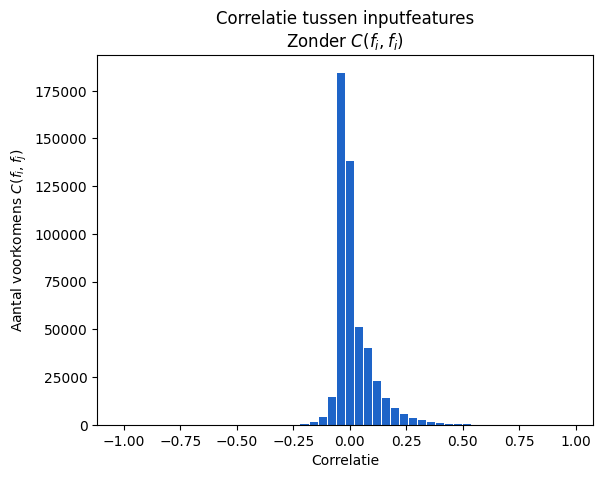
\includegraphics[width=1\linewidth]{fig/chapt4/NLP/correlaties_input.png}
        \caption{Histogram correlaties tussen inputfeatures}
        \label{fig:chapt4_correlaties_input}
    \end{subfigure}
    \begin{subfigure}{.5\textwidth}
        \centering
        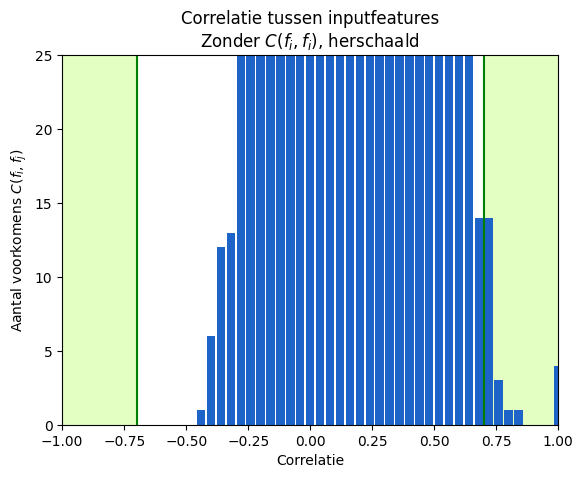
\includegraphics[width=1\linewidth]{fig/chapt4/NLP/correlaties_input_herschaald.png}
        \caption{Histogram correlaties tussen inputfeatures, herschaald voor randwaarden}
        \label{fig:correlaties_input_herschaald}
    \end{subfigure}
    \caption{Analyse correlaties inputfeatures}
    \label{fig:chapt4_correlaties_combined}
\end{figure}

\begin{table}[H]
    \centering
    \begin{tabular}{l|l}
    Feature 1 & Feature 2 \\ \hline
    restaurant category nightlife & restaurant category bars \\
    restaurant category event planning \& services & restaurant category caterers \\
    restaurant category beer & restaurant category wine \& spirits \\
    restaurant category music venues & restaurant category arts \& entertainment \\
    restaurant NLP profile 37 & restaurant NLP profile 17 \\
    restaurant NLP profile 323 & restaurant NLP profile 180 \\
    user compliments & user fans \\
    user positive interactions & user fans \\
    user positive interactions & user compliments \\
    user category nightlife & user category bars \\
    user category japanese & user category sushi bars \\
    user category event planning \& services & user category caterers \\
    user category beer & user category wine \& spirits \\
    user category music venues & user category arts \& entertainment \\
    \end{tabular}
    \caption{Paren van features waarbij de absolute waarde van de correlatie groter is dan $0,70$}
    \label{}
\end{table}

De volledige data is beschikbaar in \verb|src/corr.zip|. Deze conclusie geldt voor alle varianten van profielen gemaakt door NLP.

\subsection{Testset-up}
De modellen zijn steeds geschreven in Python 3.10. De implementaties maken gebruik van PyTorch 2.0.0. \cite{pytorch} De inputvector voor het neuraal netwerk bestaat uit \verb||torch.float32 getallen. De uitvoering gebeurt op een AMD Ryzen 5800X, NVIDIA RTX 2080, en 64GB werkgeheugen.

In dit deelonderzoek evalueren we de architectuur en parameters van het neuraal netwerk. Het effect van de inhoud van de inputvectoren wordt niet verder onderzocht. Zoals besproken in \autoref{sub:chapt4_testsetup}, zijn er meerdere mogelijke combinaties voor de NLP-profielen. We kozen de beste combinatie van profielen om verder mee te experimenteren. We analyseren iedere implementatie op dezelfde manier. De data wordt verwerkt zoals beschreven in \autoref{sec:chapt4_data_flow}: iedere epoch trainen we het neuraal netwerk met een trainset en berekenen we vervolgens de loss op de testset. Als de loss meerdere epochs op rij omhoog gaat, stoppen we het trainen om overfitting te voorkomen. De gebruikte lossfunctie voor optimalisatie is de MSE.

Nadat het model volledig getraind en getest is volgens de hierboven beschreven methode, analyseren we het model aan de hand van voorspellingen zoals we ze in de praktijk zouden gebruiken: we nemen een subset van de testset om aan de hand van het model een score tussen 1 en 5 te voorspellen. We ronden hierbij de voorspelling af, zodat het domein van de voorspelde score exact overeenkomt met het domein dat een gebruiker heeft op Yelp. We maken een histogram van het verschil tussen de voorspelling en echte score toegekend door de gebruiker. Dit histogram gebruiken we als controle dat een lagere MSE overeenkomt met meer accurate voorspellingen.

\subsection{Basisimplementatie}
\label{sec:chapt4_basisimplementatie}
We beginnen met een basisimplementatie van een neuraal netwerk, om te verifiëren dat het mogelijk is om de echte score te schatten op basis van de inputdata. We werken met een standaard multilayer perceptron (feed-forward) model. De output van het model is één waarde in $[0, 1]$. We implementeren het aanbevelingssysteem dus als een regressiemodel, waarbij de output daarna herschaald wordt naar een score tussen 1 en 5. We kiezen voor de bij regressiemodellen veelgebruikte lossfunctie MSE. Deze is ook makkelijk om te zetten naar RMSE, wat vergelijken met andere onderzoeken rechtdoorzee maakt. \cite{narre, deepconn, wide_deep_learning_paper}

Het model bestaat uit 5 verborgen lagen, waarbij het aantal neurons eerst stijgt en daarna steeds halveert (\autoref{fig:chapt4_basisimplementatie}). In tegenstelling tot collaborative filtering, kan dit model wel niet-lineaire verbanden capteren. We gebruiken Stochastic Gradient Descent (SGD) als netwerkoptimizer, met een learning rate van $0,01$.

\mijnfiguur[H]{width=16cm}{fig/chapt4/predictor/basisimplementatie_netwerk.png}{Voorstelling basisimplementatie, waarbij $n$ het aantal inputfeatures voorstelt}{fig:chapt4_basisimplementatie}



\subsection{Uitbreidingen architectuur}
We blijven bij een standaard feed-forward multilayer perceptronmodel. Dit is de meest logische keuze voor deze context. Er is bijvoorbeeld geen nood aan een model met geheugen zoals LSTM daar de inputdata geen volgorde bevat. 
We onderzoeken wel het aantal lagen en het aantal neuronen per laag. Hoe complexer het netwerk, hoe meer verbanden het capteren. Echter zorgt een stijging in complexiteit van het netwerk ook voor een complexere training die meer data nodig heeft. Complexere netwerken scoren ook slechter bij explainability. Daarom voeren we experimenten uit met een eenvoudiger netwerk met maar 1 verborgen laag, tot 8 verborgen lagen. Deze netwerken volgen een analoge structuur zoals beschreven in \autoref{sec:chapt4_basisimplementatie}. Vanaf 5 verborgen lagen zal de eerste verborgen laag wel $20$\% groter zijn dan de inputlaag, om het netwerk de kans te geven om complexere verbanden te modelleren. Tussen de eerste drie verborgen lagen zit steeds een dropout-laag. Deze laag heeft een 20\% kans om een neuron op 0 te zetten en helpt zo om overfitting te voorkomen. \cite{nn_dropout} Tijdens het testen van het model worden deze dropout-lagen uitgezet.

\subsection{Optimalisaties}
\subsubsection{Netwerk-optimizer}
We onderzoeken welk effect de gekozen optimizer heeft op de loss van het netwerk. SGD is een relatief eenvoudige optimizer waarbij de learning rate constant blijft. We proberen ook ADAGRAD, omdat deze optimizer de mogelijkheid biedt om de initiële learning rate aan te passen naargelang het trainen vordert.

De lossfunctie duidt de fout aan zodat de optimizer weet hoe het netwerk aan te passen. We onderzoeken verschillende lossfuncties die gebruikt worden tijdens het trainen, en analyseren of het resulterende model beter presteert. Het idee is dat met een aangepaste lossfunctie we beter kunnen aanduiden welk type fouten we willen voorkomen. Zo kunnen we bijvoorbeeld een exponentieel grotere fout toekennen aan voorspellingen die slechte restaurants toch inschatten als een goede match. Dit is een scenario dat we in de praktijk willen voorkomen: het is beter dat een gebruiker het perfecte 5-ster restaurant mist dan dat een 1-ster restaurant wordt aanbevolen.

\subsection{Invloeden dataset}
De Yelp dataset bevat in totaal 4 731 031 reviews over restaurants, waarbij veel gebruikers slechts één review hebben nagelaten. We bekijken in welke mate het Cold-Startprobleem een impact heeft op de betrouwbaarheid van het aanbevelingssysteem. Dit doen we door de gebruikers op te splitsen in partities gebaseerd op aantal reviews. We meten dan de accuraatheid per review.\newline
Neurale netwerken zijn vaak onstabiel bij kleinere datasets. We onderzoeken wat de impact is van het verwijderen van een deel van de dataset.\newline
We bestuderen ook of het verwerken van de tekstuele data tot profielen een meerwaarde is voor het voorspellingsvermogen van het netwerk, en of een dimensionaliteitsreductiealgoritme de grootte van de inputlaag van het model efficiënt kan beperken, waardoor het model makkelijker te trainen valt. Als de inputdata beschreven is in een lagere dimensie, dan is het eenvoudiger om generaliteit aan te leren aan het model. \cite{curse_of_dim}

\section{Andere implementaties}
We vergelijken ons neuraal netwerk met een baseline methode die steeds 4 sterren voorspelt, en met traditionele methoden: Content-Based Filtering en User-User/Item-Item Collaborative Filtering. We vergelijken ons model ook met state-of-the-arttechnieken: DeepCoNN en Wide \& Deep Learning.\newline
Van alle implementaties heeft een neuraal netwerk het meeste potentieel om de hoogste precisie te halen, ten koste van explainability. We onderzoeken hoeveel precisie we opgeven als we een random forest-architectuur gebruiken in plaats van een neuraal netwerk.
